\section{Statistical postulates}
So far we have looked at the macroscopic properties of a thermodynamical system and at some ways of calculating properties of random processes that obey some given probability distribution. Now it is time to combine these ideas and have a first attempt at linking the microscopic behaviour of a thermodynamic system (an idealised gas) with some of its macroscopic properties.

The behaviour of a given (mechanical) system depends on both the structure of the system --- described by its equations of motion --- and on the \emph{initial conditions} of the system. Therefore, in order to describe the behaviour of the system, we need both the laws of mechanics for the system along with some statistical postulates about the initial conditions of the system. (We could also require that we know the exact initial conditions for all the particles in the system, but this is not realistic for $\mathcal{O}(10^{23})$ particles.) Different choices of the statistical postulates can lead to different behaviour (not just different states) of the system. We will look at Maxwell's postulates for the initial positions and velocities of a dilute collection of gas particles. We will see that they allow us to derive the ideal gas law from a microscopic basis.

\subsection{An ideal gas}
We want to keep the equations of motion for our system of particles as simple as possible. We are going to assume   that our system has the following properties:
\begin{itemize}
\item We have $N$ identical  point particles, each with mass $m$, constrained in a volume $V$.
\item There are no mutual interactions --- no van der Waals effects or inter-particle forces for us!
\item The walls of the container constraining the particles are perfectly reflecting.
\item The mechanical state of the system is known when the position $\bf r$ and velocity $\bf v$ is known for each particle and these variables evolve according to Newton's laws of motion.
\end{itemize}

\subsection{Maxwell's postulates}
Maxwell's postulates translate the ideal gas assumptions from the previous section into conditions that we can use with Newton's equations of motion in order to, in principle, describe everything about the behaviour of an ideal gas. From these we can infer macroscopic properties by simply integrating over the microscopic variables of the system.

We assume that the vectors describing the initial conditions of the system are randomly distributed. More specifically:
\begin{enumerate}
\item The vectors relating to each particle are independent from each other. (e.g. there is no interaction between particles when they are close.) This is generally not true for any but the most dilute systems. For such a non-interacting system, the system's state is determined when $dN=f({\bf r},{\bf v})$ is known, where $dN$ is the number of particles in a box with sides $d{\bf r}=(dx,dy,dz)$ centered on the point ${\bf r} = (x,y,z)$ and where the corresponding velocities of the particles lie within a box d${\bf v}=(dv_x,dv_y,dv_z)$ centered on ${\bf v}=(v_x,v_y,v_z)$. This relationship defines the \emph{single-particle distribution} $f({\bf r},{\bf v})$.
\item The positions ${\bf r}$ are independent of the velocities ${\bf v}$. This means we can factorise $f({\bf r},{\bf v})$ as $f({\bf r},{\bf v})$ =$f_r({\bf r})$ $f_v({\bf v})$ .
\item The density of the gas is uniform within the volume so we can write $f({\bf r}) = N/V=\rho=$ constant inside the volume (and zero outside it).
\item The velocity components are independent of each other so we can factorise $f_v$ as $f_v({\bf v})=f_x(v_x)f_y(v_y)f_z(v_z)$.
\item The distribution $f_v({\bf v})$ is isotropic in velocity space so that $f_v$ depends only on the magnitude of the velocity $|{\bf v}| = v$
\end{enumerate}

\subsection{Micro to Macro}
Using the postulates above, we can derive a macroscopic equation of state. We will prove that Maxwell's postulates will allow us to derive the equation of state for ideal gases.
\begin{figure}[H]
	\begin{center}
		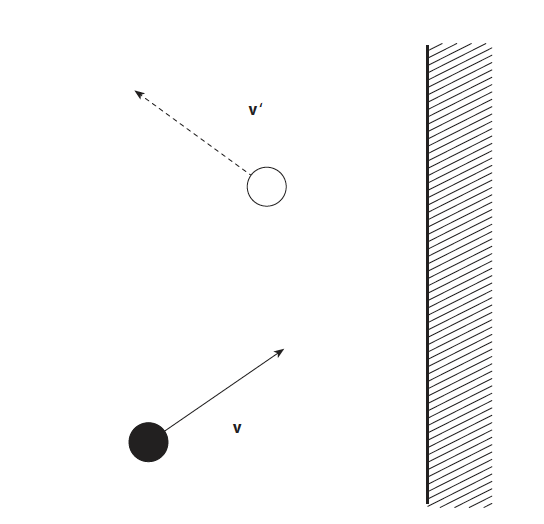
\includegraphics[width=0.4\textwidth]{bouncyboi}
	\end{center}
	\caption{Particle impacting a wall}
\end{figure}
Consider a particle with velocity ${\bf v} = (v_x,v_y,v_z)$, moving from the left, that hits a wall parallel to the $yz$-plane. After impact its velocity is ${\bf v'}=(-v_x,v_y,v_z)$. Hence, the change in momentum is $\Delta {\bf p}= {\bf p'} - {\bf p} = m({\bf v'}-{\bf v}) = m(-2v_x,0,0)$.

How many such impacts occur in a given time interval $\Delta t$ on a region of the wall with area $A$? 
Take a box with a side of area $A$ on the wall and perpendicular sides of length $v_x\Delta t$. This contains the particles of velocity ${\bf v}$ that can hit the wall. The volume of the box is $Av_x\Delta t$ and the number of particles it contains is $\rho Av_x\Delta t f_v({\bf v})$, where $\rho=N/V$ is the density of all particles  and $f_v$ is the probability that a particle has velocity $\bf v$.
The total momentum $\Delta P$ transmitted to the wall is therefore
$$\Delta P =\int_0^\infty dv_x \int_{-\infty}^\infty dv_y \int_{-\infty}^\infty dv_z f_v({\bf v})\rho A\Delta t(-2m)v_x^2{\bf i}$$
where ${\bf i} =(1,0,0)$ picks out the $x$-component. i.e. integrate over the number of particles times the momentum per particle. The first integral only runs from zero since we are only interested in particles traveling towards the right, i.e. ${\bf v}>0$. The factor of $\frac{1}{2}$ comes from integration over $v_{x}$, which runs only from $v_{x} > 0$.

The integral above gives 
$$\Delta P = -2m\rho A\Delta t \langle v_x^2\rangle\frac12$$ where the average square velocities come from integrating over the velocity distribution and the factor of half comes from the integral over $v_x$, i.e. particles moving towards the right.

The force exerted by the gas on the wall is $F=\Delta P/\Delta t$ and pressure is force/area = $|F|/A$.
We therefore have 

\begin{equation}
	p=m\rho  \langle v_x^2\rangle.
	\label{eq1.2}
\end{equation}
 
Compare this with the classical equation of state for an ideal gas $pV=NK_BT$ where $T$ is the absolute temperature and $k_B=R/N_A$ is Boltzmann's constant ($R\simeq8.3JK^{-1} \text{ mol}^{-1}$ is the ideal gas constant and $N_A\simeq6\times10^{23}mol^{-1}$ is Avogadro's number). Since $\rho = N/V$, equation \ref{eq1.2} suggests that we can relate the absolute temperature $T$ to the mean square velocities of the particles (times a constant).
\begin{align*}
	p &= \rho k_{B}T
\end{align*}


